% !Mode:: "TeX:UTF-8"
\chapter{基于大模型的表格数据检索增强与推理优化}
\label{cha:第四章}
本章节主要以大模型在表格数据推理以及实际应用场景进行了深入的研究,提出了一种多级表格检索增强方法和大模型的表格推理框架,解决了检索增强推理任务中对表格文件的召回率低和大模型对表格数据推理能力差的问题。并将其应用于水利水库调度业务场景,构建水利水库调度场景下的基于大模型的智能反馈交互系统。
\section{问题描述}
结构化表格数据作为信息组织与存储的关键形式,在企业数据库、科研记录、金融报表等诸多领域有着广泛且深入的应用。在当今数字化转型加速的时代背景下,数据驱动的决策制定、业务流程优化以及知识发现等活动,愈发依赖于对结构化表格数据的高效利用与深度挖掘。

大型语言模型(LLMs)凭借其强大的语言理解和生成能力,已经在自然语言处理领域取得了显著成就。然而,传统LLMs在处理结构化表格数据时存在明显局限性,主要表现为对表格数据的结构化特征理解不足,难以有效执行复杂的数值计算、数据关联以及逻辑推理等任务。这在很大程度上限制了LLMs在众多实际应用场景中的进一步拓展与深化。这种能力的提升对于拓展大模型在真实场景中的实用性具有至关重要的意义。在数据分析方面,模型可以更高效地从海量表格数据中提取有价值信息,生成具有深度理解的分析报告;在决策支持场景中,模型则能够基于表格数据进行复杂的情景模拟与预测分析,为决策者提供科学、可靠的依据,助力其做出更明智的决策。
\section{表格数据推理框架的搭建}
表格数据具有复杂的行列关系、数值精度高、规模庞大等特点,传统LLM易受上下文长度限制、高token消耗和数字语义解析能力不足的影响。研究大模型表格推理方法(如程序生成、检索增强)能有效解决这些问题,提升模型对结构化信息的处理效率和能力。目前主流的大模型表格数据推理方法是借助代理Agent思想,将问题中的数据分析任务和语义理解等任务剥离,将任务拆分为各个子任务,代码生成任务为最关键的一步,根据任务需要生成可执行的代码,再通过外部接口对表格执行如SQL、python等机器语言来简化表格内容,降低任务难度,进而提升大模型对表格推理能力。

该研究主要面临两个困难和挑战,首先是大模型对数字文本的理解推理能力不足,如图\ref{fig:4-1}所示,大模型无法理解多个数据之间的数量大小关系,无法进行准确的数学计算,以至于对关键数字信息的提取和处理出现错误;二是对于庞大的表格数据,直接将结构化表格文本线性化的方法会产生过长的上下文,从而超出模型的最大上下文长度,从而截断表格,导致信息缺失降低回答质量。并且大模型处理过于复杂和冗长的上下文信息时,会因为无法识别关键信息而出现幻觉问题。综上所述,要提高大模型对表格数据的处理能力需要完成两个工作,一是将表格中复杂的数据关系和计算任务通过外部工具实现,二是剔除表格中与问题无关的冗余数据,只留下关键数据降低推理负担,从而提高大模型的推理能力。
\begin{figure}[!htbp]
    \centering
    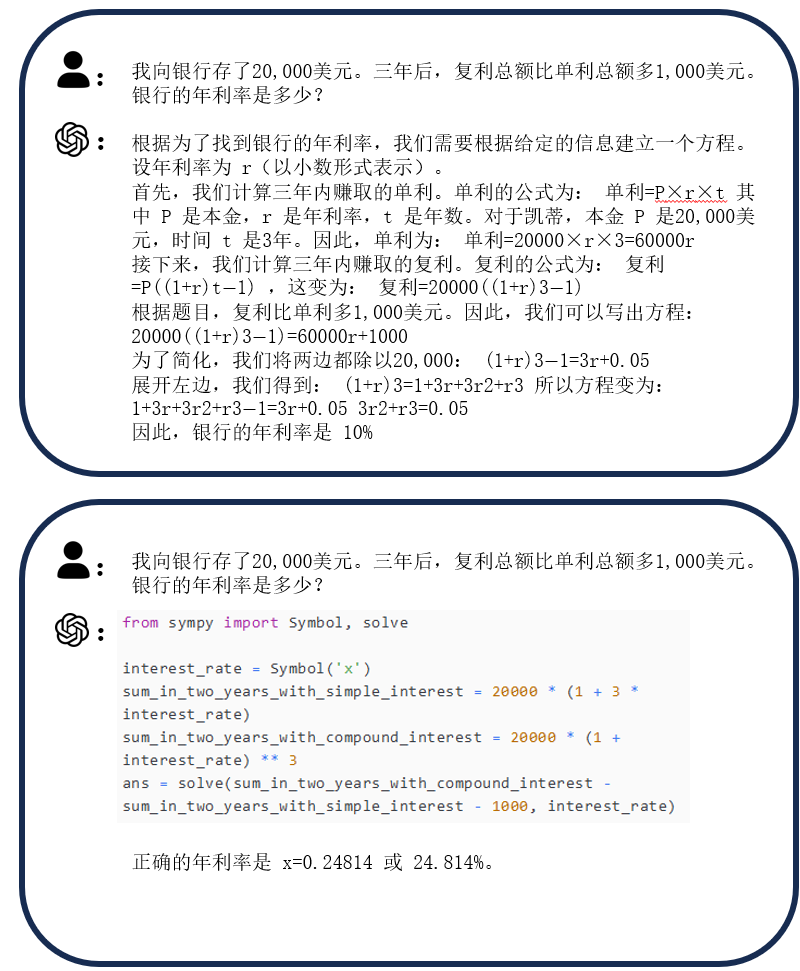
\includegraphics[width=0.7\textwidth]{大模型对数学问题的处理结果.png}
    \bicaption{大模型对数学问题的处理结果}{Results of Mathematical Problem Processing by LLM}
    \label{fig:4-1}
\end{figure}
同时,面对实际数据分析任务,表格数据输入模态多种多样包括excel表格、纯文本形式表格、数据库database表格和PDF表格等。针对多模态的表格文件主要存在两种处理方式,一种是将所有模态表格均以图片的形式输入大模型\cite{zhengMultimodalTableUnderstanding2024},利用了LLaVA、Vit\cite{bangMultitaskMultilingualMultimodal2023,chenCLIP2SceneLabelefficient3D2023,liuVisualInstructionTuning2023,radfordLearningTransferableVisual2021,dosovitskiyImageWorth16x162020}等视觉编码模型将表格编码输入大模型,是一种端到端的方法,该方法即使在部分任务的表现上达到了最优,但是该方法缺乏可解释性、消耗计算资源过于庞大且依然不能解决大模型对数字信息的计算和推理能力;第二种方法是利用Agent代理的思想,利用外部接口来代替大模型处理数学问题并简化表格文件,提取关键信息。利用代理思想的方法拓展了大模型在解决问题时的功能多样性,将多种大模型不熟悉的如数字运算、数字推理等任务统一转化成代码生成任务,即大模型最擅长的任务。代理方法相对视觉编码的方法节约了大量训练算力,并且提高了大模型在任务中的可观测性和可解释性,是实际应用中的主流方法。
\subsection{多级表格数据检索构建}
该方法主要包括对复杂表格数据的预处理、大模型的多轮推理以及外部SQL接口的使用。目前的主流表格推理框架默认所推理表格与问题的相关性,直接将具备回答问题所需信息的表格作为输入,测试框架的推理能力。但是在实际的推理任务中,需要通过文本向量相似性等方法对目标表格进行召回,为了提高召回精度同时保证大模型的推理的后续推理能够顺利进行,下面本章节提出一种多级表格数据目录检索方法。

由于表格数据的数据结构特点,使用RAG系统中传统的文本预处理切块方式会导致表格的召回率不高和召回表格不完整。对于传统文件处理方式,将表格数据以文本方式使用切块方法将表格以多个文本块的形式向量化存储在向量数据库中。由于表格文件的大部分信息均为数字,如果表格在中间截断,表格的中间部分以响亮的形式存在,没有表头和表名,数据会丧失意义和信息。同样不同表格的中间数据部分会有相似的情况,若直接使用文本相似度检索非常容易将不同表格的数据信息混淆,导致信息失真,进而影响回答质量。表格数据之间相互区别的主要信息主要为表名和表头,这两个特征赋予数字实际意义,所以希望根据表头和表名信息构建数据向量库,同时也能够避免表格数据因长度过长被分割后,单独的数字信息丧失实际意义的问题。同时将过长的表格数据存储在向量数据库中也会在召回时浪费大量的相似度计算资源和延长响应时间。综上所述,本文设计了只将表名和表头向量化存储在向量数据库中,把表格的数据信息通过JSON和database的形式存储在本地,根据向量化检索后的metadata进行本地表格定位,并且根据不同表的特征进行优化的表格召回方法。该方法可以提高召回率和召回效率,并且可以保证将完整表格输入给大模型推理,同时为后续推理优化方法提供了格式化的表格文件。
\begin{figure}[!htbp]
    \centering
    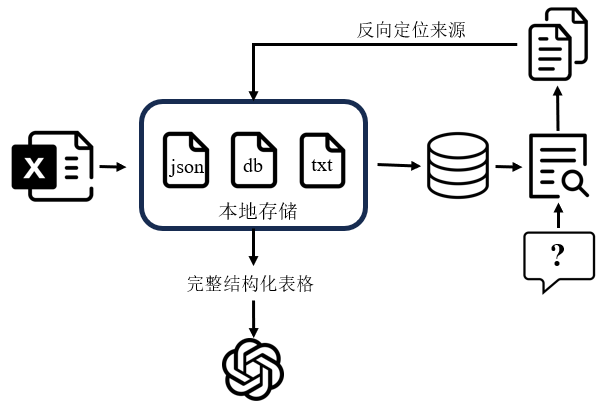
\includegraphics[width=0.66\textwidth]{表格检索框架示意图.png}
    \bicaption{表格检索框架示意图}{Schematic Diagram of Table Retrieval Method}
    \label{fig:4-2}
\end{figure}
将表格文件转化为JSON、database和txt文本形式存储,再将txt文件中的表名和表头文本嵌入向量化,此时在向量数据库中,每一条对应的表头信息都包含一个特征metadata,即这个向量数据是由哪个文件向量化而来。当输入的问题通过向量搜索模型匹配到目标表格时会直接定位到本地原始文件,根据需要提供JSON文件和database文件给后续框架进行推理等操作。在向量检索中使用双塔检索结构\cite{bahdanauNeuralMachineTranslation2016,sutskeverSequenceSequenceLearning2014,radfordImprovingLanguageUnderstanding2018,fanHierarchicalNeuralStory2018,holtzmanCuriousCaseNeural2020}。在召回过程中,双塔检索结构通过分阶段优化效率与精度,通常分为粗召回(Candidate Generation)和精排序(Re-ranking)两个层级:粗召回阶段采用双塔神经网络架构,其中查询侧(Query Tower)和候选侧(Item Tower)分别通过独立编码器如Transformer,将问题文本编码为词向量,其中候选侧的编码过程为离线进行,在向量库构建时完成。再通过向量内积或余弦相似度计算初步匹配得分,并借助近似最近邻搜索(ANN)快速筛选Top-K候选集,实现计算效率与召回覆盖率的平衡;精排序阶段则引入复杂模型如第\ref{chap:第二章}章中介绍的BERT模型,对粗召回结果进行精细化相关性评估与排序,直接通过端到端的方式将问题和粗召回的候选向量输入,由模型输出相似度得分,从而在可控计算成本下提升整体召回质量。两阶段分工耦合,形成“高效粗筛-精准判别”的递进式检索范式,兼顾系统响应速度与语义匹配深度。由于向量库中的数据庞大,如果直接使用端到端方式筛选合适文本表格会耗费大量的计算资源和时间,所以会提前通过比较文本相似的的方式以离线的方式将数据嵌入,但只依赖这种方法无法保证搜索到准确性,所以使用了先召回后精排的搜索方式。
\subsection{循环推理框架构建}
如上文提到,如果直接将上小节引入的检索方法检索到的表格输入给大模型会存在表格过长超出模型最大上下文长度和大模型对表格数据推理能力差的问题。可以通过引入Agent代理思想,通过SQL执行来处理表格,通过将数据精简减少表格长度和推理难度的方式提高回答质量,同时也使用SQL的计算能力来弥补大模型对数字关系推理的不足。

Agent代理的核心思想之一是将复杂任务分解为多个简单任务,从而降低每一次大模型调用时面对任务的难度,进而提升回答质量。是由多个大模型分工合作共同完成一次推理任务。综上所述,提出一种大模型循环表格推理框架,利用大模型强大的代码生成能力和自纠错能力生成准确有意义的SQL代码,再由外部接口执行代码并循环以上操作,得到最后精简的数据供大模型推理生成最终答案。

单次调用大模型生成SQL结果需要统一格式并且尽量降低模型的输出丰富度,可以通过调整模型输入参数和设计特殊提示词模板来实现,模型可以通过temperature参数控制输出的丰富程度,temperature越高,生成的文本更多样,反之,生成的文本更确定,因此对于生成SQL的大模型temperature设置为0.8,因为既需要固定同一个表格同一个需求输出SQL的一致性,也需要适当提高针对同一个表格不同需求的多样性。而针对固定大模型的输出格式上,框架希望可以直接将输出的文本作为下一阶段推理的输入,所以需要输出为可直接运行的SQL代码。上述需求通过提示词来解决。

提示词作为大模型调用的关键一环,可以不经过训练只使用文字输入的形式让大模型了解任务的需求,具体原理介绍已经在第\ref{chap:第二章}章写明。在SQL生成的提示词中,需要满足以下要点:

首先明确提出任务需求,该大模型的推理任务是什么。其次令模型理解输入的表格具体结构。因为检索到的目标表格也是以提示词的形式作为输入给大模型,这涉及到上面提到的表格篇幅过长问题,既需要令大模型明白表格的全貌,又需要减少表格长度。这里同样借助SQL的能力,利用SQL中表格初始化代码代替整张表格来使大模型理解表格结构,同时将大模型的知识注意力引入SQL中,再截取表头和少量表格信息组成提示词。在生成可直接运行的SQL代码的过程中,若采用冗长的文本描述方法,会存在以下问题:一方面受限于文字表达能力的局限性,难以精准且简洁地描述SQL代码的生成逻辑与结构;另一方面,模型在理解与转化这些文本描述时,存在一定概率出现语义对齐不准确的问题,导致生成的SQL代码无法准确实现预期功能。为解决这一问题使用Few-shot learning少样本学习方法,通过少数训练样本直接以提示词的形式来规范输出格式。设计满足以上需求的提示词如图\ref{fig:4-3}所示。
\begin{figure}[!htbp]
    \centering
    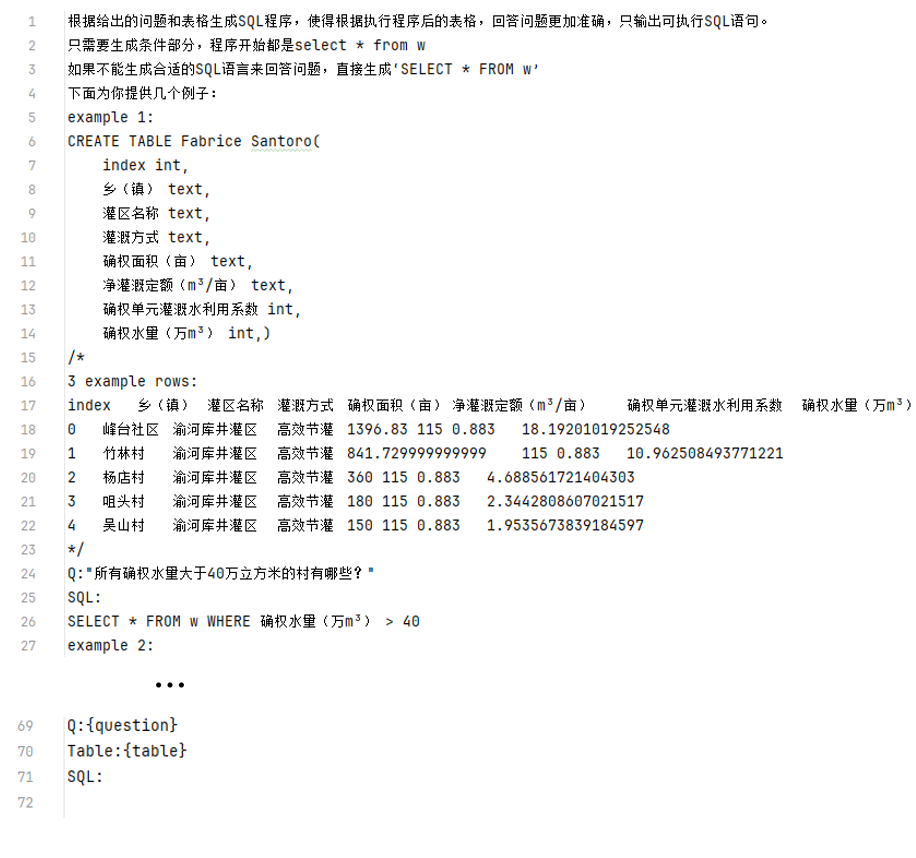
\includegraphics[width=0.95\textwidth]{SQL生成任务提示词.png}
    \bicaption{SQL生成任务提示词}{SQL Generation Task Prompt Words}
    \label{fig:4-3}
\end{figure}

提示词模板最后通过字典的格式将问题和文本化表格嵌入,由于少量输入输出例子,大模型会优先模仿并跟随前面的输出,就能保证输出SQL语句的一致性。
\begin{figure}[!htbp]
    \centering
    \includegraphics[width=0.79\textwidth]{无few-shot.png}
    \bicaption{无少样本学习的SQL生成}{ SQL generation without Few-shot learning}
    \label{fig:4-4}
\end{figure}
特别注意的是,嵌入提示词模板的表格数据都将是以图\ref{fig:4-3}中一样文本的形式,包括最后生成回答的推理过程,database的文件形式只用于在框架内部利用SQL生成简化后的表格。然而还是有概率会出现输出SQL命令执行出错的问题如下图\ref{fig:4-5}所示。这里需要利用大模型的代码理解能力与自纠错能力,设计一种大模型的多循环自反馈框架。
\begin{figure}[!htbp]
    \centering
    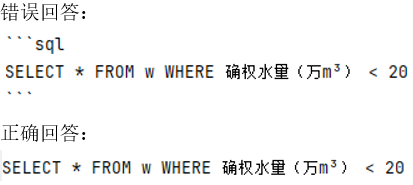
\includegraphics[width=0.5\textwidth]{SQL生成对比.png}
    \bicaption{SQL生成对比}{Comparison of SQL Generation}
    \label{fig:4-5}
\end{figure}

该框架中设计的为三次循环反馈的自适应错误修正框架,其核心机制在于构建动态上下文感知的自纠正系统。将每次执行输出报错后的系统报错与前文组成上下文,生成包含完整错误的增强型上下文再输入模型。经过实际测试,将往次输入的报错和纠正共同组成上下文输入给模型非常关键,这样有助于令大模型意识到自身的错误方向和改进方向,若每次的报错信息单独输入给大模型会导致其原地踏步,孤立地处理离散错误事件。
\begin{figure}[!htb]
    \centering
    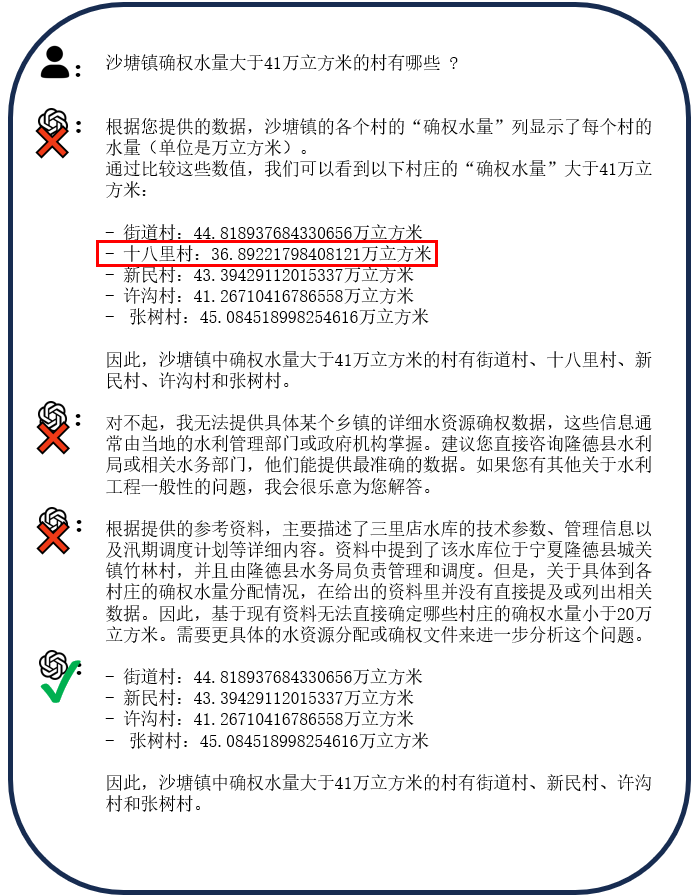
\includegraphics[width=0.8\textwidth]{回答对比.png}
    \bicaption{优化前后回答对比}{ Comparison of Answers Before and After Optimization}
    \label{fig:4-7}
\end{figure}
当系统经历完整的三次迭代仍未能达成有效修正时,系统自动切换至为无优化的基础查询模式,直接执行select * from w全表扫描指令,将全部表格输出给下一步推理,来确保系统输出的完整性。这种双重模式切换机制在保证框架鲁棒性的同时,有效规避了因循环修正导致的潜在计算资源浪费问题。整体过程如图\ref{fig:4-6}所示。
\begin{figure}[htbp]
    \centering
    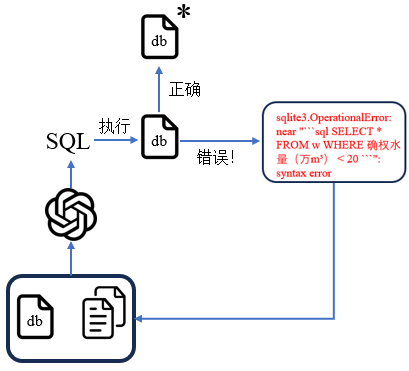
\includegraphics[width=0.63\textwidth]{循环反馈示意图.png}
    \bicaption{循环反馈示意图}{Schematic Diagram of Feedback Loop}
    \label{fig:4-6}
\end{figure}

\section{反馈信息优化对比}
针对表格检索任务,由水利局专家设计构造了针对隆德水库信息查询的问题集并对本章提出的多级表格检索方法和不进行特殊处理直接使用FAISS内部向量化嵌入方法进行对比测试。在测试中为了避免表格超出上下文长度导致的表格截断问题,只统计在大模型最大上下文长度内的表格与对应问题,测试结果如表\ref{tab:table-retrival-results}所示。
根据实验结果显示,本章提出的多级表格检索方法在召回率上有明显提升,提高了表格数据的召回率。同时也针对SQL的生成任务做出了测试,通过专家对测试结果的评估判断是否能够生成可执行、有优化效果的SQL。在实验中对于直接生成方式也进行了提示词辅助生成,测试结果如表\ref{tab:SQL-Generation-results}所示,其中SQL生成正确率代表框架生成的能够正确执行的SQL比例,SQL生成恰当率代表框架生成的能够优化表格的SQL比例。

针对后续模型推理回答效果的测试,通过一个信息查询任务回答展示具体效果,如图\ref{fig:4-7}所示。测试涉及对目标表格“隆德县农业灌溉用水确权汇总表”的召回和单特征数量关系的筛选。第一个回答为返回目标表格但无SQL优化回答,在回答中出现了错误答案,误将确权水量为36万立方米的十八里村输出;第二个回答由于在召回过程中,所有的向量相似度过低没有达到阈值,无表格返回;第三个回答为返回错误表格“三里店水库汛期调度运用计划表”导致;最后的回答为通过优化方法正确召回目标表格并使用推理框架得到正确数据的结果。由于最后输入给模型推理的表格只有符合要求的数据,所以避免了模型对数量关系不敏感的缺点,实现回答效果优化。
\begin{table}[h]
    \centering
    \bicaption{表格检索实验结果}{Table Retrieval Experiment Results}
    \label{tab:table-retrival-results}
    \begin{tabularx}{\linewidth}{XXX}
        \toprule[1.5pt]
        {方法} & {原始方法} & {多级表格检索方法} \\
        \midrule[1pt]
        {召回率} & 66.3\% & 80.9\% \\
        \bottomrule[1.5pt]
    \end{tabularx}
\end{table}
\begin{table}[h]
    \centering
    \bicaption{SQL生成实验结果}{SQL Generation Experiment Results}
    \label{tab:SQL-Generation-results}
    \begin{tabularx}{\linewidth}{XXX}
        \toprule[1.5pt]
        {方法} & {直接生成} & {循环推理框架} \\
        \midrule[1pt]
        {SQL生成正确率} & 46.3\% & 60.9\% \\
        {SQL生成恰当率} & 30.9\% & 52.7\% \\
        \bottomrule[1.5pt]
    \end{tabularx}
\end{table}
\section{本章小结}
本章节主要探讨了基于大模型的表格数据推理框架的设计,旨在提升大模型对结构化表格数据的理解与推理能力。通过深入分析表格数据的特点及大模型在处理表格数据时面临的挑战,提出了一种结合多级表格数据检索与循环推理的框架。

首先,针对表格数据的复杂性和大模型的局限性,设计了一种多级表格数据检索方法。该方法通过将表格的表名和表头信息向量化存储,避免了表格数据因长度过长而被分割的问题,提高了表格数据的召回率和召回效率。
其次,提出了一种大模型循环推理框架,通过引入Agent代理思想,将复杂任务分解为多个简单任务,降低了每次大模型调用时的推理难度。该框架利用大模型的代码生成能力,生成可执行的SQL代码,通过外部接口执行代码来简化表格数据,弥补了大模型在数字推理能力上的不足。此外,设计了一种多循环自反馈机制,通过动态上下文感知的自纠正系统,提高了推理的准确性和鲁棒性。

通过上述方法,本章成功构建了一个高效的表格数据推理框架,显著提升了大模型在处理结构化表格数据时的性能。这一框架不仅优化了表格数据的检索和推理过程,还为实际应用中的智能反馈交互系统提供了强有力的技术支持。

本章所述内容已应用于学校合作企业的相关技术研发,并已提交专利申请。
